\documentclass[preprint,12pt]{elsarticle}
\usepackage[
  backend=biber,
  style=numeric,
  sorting=none,
  maxbibnames=99
]{biblatex}
\addbibresource{reference.bib}

% -------- Encoding & fonts (pdfLaTeX) --------
\usepackage[utf8]{inputenc}
\usepackage[T1]{fontenc}
\usepackage{textcomp}
\usepackage{microtype}
\usepackage{newunicodechar}
\newunicodechar{−}{-}
\usepackage[utf8]{inputenc}
% -------- Math & symbols --------
\usepackage{amsmath, amssymb}
\usepackage{booktabs}
\usepackage{siunitx}
\sisetup{
  detect-weight=true,
  detect-inline-weight=math,
  round-mode=places,
  round-precision=2,   % ← exactly two decimals
  fixed-exponent=0
}


% -------- Hyperlinks & URLs --------
\usepackage[hidelinks]{hyperref}
\usepackage{url}

% -------- Graphics & figures --------

\usepackage{graphicx}
\usepackage{caption}
\usepackage{subcaption} % sub-panels
% subcaption + some classes sometimes need this for older packages:
\captionsetup{compatibility=false}


\graphicspath{
  {../figures/}
  {../pic/}
  {figures/}
  {pic/}
  {results/uncertainity_figures/ready/}
  {results/uncertainity_figures/ready/groups/}
  {results/uncertainity_figures/ready/before_after/}
  {results/uncertainity_figures/ready/cross_group/}
  {results/uncertainity_figures/ready_numbers/}
  {results/Paper_A/}
  {results/Paper_A/A_Appendix/}
  {results/}
}
\DeclareGraphicsExtensions{.pdf,.png,.jpg,.jpeg}

% -------- TikZ for diagrams --------
\usepackage{tikz}
\usetikzlibrary{shapes.geometric, arrows.meta, positioning}

% -------- Tables --------
\usepackage{array, booktabs, tabularx, adjustbox}
\usepackage{siunitx}
\sisetup{round-mode=places, round-precision=3, detect-all}
\newcolumntype{Y}{>{\raggedright\arraybackslash}X}
\newcolumntype{Z}{>{\centering\arraybackslash}X}

% -------- CSV tools (only once) --------
\usepackage{csvsimple}

% -------- ORCID badges --------
\usepackage{orcidlink}

% -------- Unicode convenience (CO$_2$ subscript 2 typed as U+2082) --------
\DeclareUnicodeCharacter{2082}{$_2$}

% -------- Line numbers (toggle) --------
\usepackage[switch]{lineno}
\newif\ifreview
\reviewfalse % set \reviewtrue for line numbers
\ifreview\linenumbers\fi

% -------- Journal name (Elsevier) --------
\journal{Environmental Modelling \& Software}

% -------- Helpers --------
\newcommand{\img}[2][\linewidth]{\includegraphics[width=#1]{#2}}
\newcommand{\safeinclude}[2][]{%
  \IfFileExists{#2}{\includegraphics[#1]{#2}}{%
    \fbox{\parbox[c][0.9in][c]{0.9\linewidth}{\centering
      \textcolor{red}{Missing figure:} \texttt{#2}}}%
  }%
}

\begin{document}

\begin{frontmatter}

\title{Pixels to pachyderms: Dual framework testing for Predicting Elephant Habitat Suitability}

\author[label1]{Harin Aiyanna C. R.\orcidlink{0009-0009-0504-1286}}
\author[label2,label3,label4]{Brooke Friswold\orcidlink{0000-0002-6484-5630}}
\author[label4,label5]{Antoinette van de Water\orcidlink{0000-0001-9410-5417}}
\author[label1,label6]{Francesco Pirotti\orcidlink{0000-0002-4796-6406}}


\affiliation[label1]{
  organization={TESAF Department of Land, Environment, Agriculture, and Forestry},
  addressline={University of Padova},
  city={Padova},
  postcode={35020},
  state={Veneto},
  country={Italy}
}
\affiliation[label2]{
  organization={Department of Wildlife Ecology and Conservation},
  addressline={University of Florida},
  city={Gainesville},
  postcode={32611},
  state={Florida},
  country={USA}
}
\affiliation[label3]{
  organization={Conservation Ecology Program},
  addressline={King Mongkut’s University of Technology Thonburi},
  city={Bangkok},
  postcode={10150},
  country={Thailand}
}
\affiliation[label4]{
  organization={Bring The Elephant Home},
  addressline={Steven Butendiekplateau 130},
  postcode={3581 GS},
  city={Utrecht},
  country={The Netherlands}
}
\affiliation[label5]{
  organization={School of Life Sciences},
  addressline={University of KwaZulu-Natal, Private Bag X01, Scottsville},
  postcode={3209},
  city={Pietermaritzburg},
  country={South Africa}
}
\affiliation[label6]{
  organization={CIRGEO Interdepartmental Research Center of Geomatics},
  addressline={University of Padova},
  city={Legnaro},
  postcode={35020},
  state={Veneto},
  country={Italy}
}



\begin{abstract}

Automated machine learning offers new opportunities to model and predict the ecological trade-offs of fencing ecology for keystone species. These structures however reveal reduction in human–wildlife conflict and yet fragment habitats essentially undermining landscape connectivity. This case study spatially analyzes the impact of fencing removal on habitat suitability and utilization for 6 elephants in the Kariega Game Reserve, South Africa. We utilized fine-scale telemetry data in conjunction with high-resolution environmental co-variates to evaluate two modeling methodologies: stacked ensemble species distribution models (SSDMs) and the h2o AutoML framework. To mitigate spatial autocorrelation, we implemented a density-based adaptive thinning algorithm (DBSCAN). Results show that the h2o AutoML approach efficiently outperformed SSDMs (AUC $\approx 0.90$ vs.\ 0.85) in predictive accuracy, highlighting the potential to scale-up automated machine learning in spatial ecology. While both frameworks agreed and captured sharper, spatially explicit habitat gradients at broad scales (Pearson's $r = 0.85$–$0.91$), AutoML revealed stronger post-fence expansion dynamics, underscoring how algorithmic flexibility shapes finer hotspot delineation. Pixel-wise difference maps based on Jaccard index effectively captured the telemetry movement patterns and fine-grained spatio-temporal change due to fence removal. We also found predicted range expansion from AutoML expanded by up to 35\% while top 25\% of both (AutoML vs SSDM) suitable pixels from the upper quartile ($J_{0.75}$), quantified as core areas. Finally, the top-ranked h2o AutoML model, selected by cross-validated area under the Receiver Operating Characteristic Curve (AUC), was projected into various climate scenarios (Shared Socioeconomic Pathways (SSPs)) to evaluate shifts in future elephant habitat utilization. The findings not only highlight an interdisciplinary machine learning approach to inform landscape delineation for keystone species conservation, but addresses value for precise modeling strategies, contributing an open framework, and comprehensive benchmarking of AutoML frameworks complementing established species distribution modeling pipelines.
\end{abstract}

\begin{graphicalabstract}
\centering

\adjustbox{width=\textheight, max width=\textwidth}{%
  \includegraphics{results/Paper A Flowchart.png}%
}
\end{graphicalabstract}

\begin{highlights}
\item Automated Machine Learning improved accuracy and spatial detail of predictions when compared to traditional SSDMs.
\item Habitat suitability shifted markedly (by up to 35\%) after fence removal for individual elephants.
\item Between-framework differences reveal uncertainty critical for conservation planning emphasizing greater efficiency
\end{highlights}

\begin{keyword}
Species Distribution Model \sep h2o AutoML \sep Habitat utilization \sep Species-Environment interactions \sep Fence removal
\end{keyword}
\end{frontmatter}

% ================= Main content =================
\section{Introduction}
\label{sec1}
Landscape restoration for the conservation of keystone species and their habitat is crucial for preserving ecological stability, biodiversity, and resilience \cite{Edwards2024} across various ecosystems. In an era of accelerating environmental change, their loss triggers cascading effects that fundamentally destabilize ecological networks and compromise essential ecosystem services \cite{Ratajczak2022,Naidoo2025,Tobias2025}. Many keystone species are becoming highly vulnerable to climate change, land-use change, and increasing human pressures \cite{Edwards2024,Kau2025}. Out of the many management interventions, fence removal stands central to the continuing debate on land sharing vs land sparing in human-wildlife coexistence \cite{Grass2019}. The most direct management challenges in southern Africa is the prevalence of wildlife fencing, established mainly to keep wildlife within the reserves while boosting eco-tourism. Although, fences following the boundary of the reserves can substantially reduce human-wildlife conflict, some internal fences may disrupt key ecological connectivity for wide-ranging animals like elephants \cite{Kremen2015,Osipova2018,Schwandner2025,Naidoo2025}.

Particularly, keystone megafauna such as African elephants, epitomize the tension between the need for conservation and landscape modification for human well-being \cite{VandeWater2024,Gross2024}. Elephants serve as ecosystem engineers, influencing biodiversity and ecological processes via seed dissemination, canopy alteration, soil and water management, and even create micro habitats \cite{Kau2025,Timteo2022}. Yet these ecosystem functions are threatened by various factors such as poaching, habitat fragmentation or degradation and climate change \cite{Nampindo2024}. Over the past fifty years, the number of savanna elephants has dropped by around 70\%, while the forest elephant populations have decreased by 90\%, leading to an estimated continental reduction of 77\% \cite{Edwards2024}. Simultaneously, atmospheric CO2 concentrations have risen to ~420 ppm, amplifying climate extremes and compounding pressures on the habitat of keystone taxa \cite{Honisch2023,Riva2024}. These combined elements make elephants not only a conservation priority but also a sensitive indicator species for assessing how landscape modifications and management interventions affect ecosystem integrity.

To quantify such changes, species distribution models (SDMs) provide a key means of linking species’ niche data with environmental variables. They provide spatial data for policymakers, reserve managers, and ecologists to assess habitat suitability, predict spatial movements, and plan conservation strategies \cite{Elith2009,Guisan2000}. High-resolution remote-sensing products, such as Sentinel-2 and MODIS, now supply continuous information on habitat data, vegetation, land cover, and human footprint. Leveraging them boosts SDM outputs to markedly improve predictive performance \cite{Agrillo2021,Jochems2024,Estopinan2022,Choe2021,Kumari2023}. Also leveraging machine learning to integrate fine scaled species occurrence data yields geographically refined forecasts that can inform proactive conservation and connection strategies \cite{Tuia2022}.

Traditionally, SDMs utilize techniques such as maximum entropy (MaxEnt), random forests, generalized linear models (GLMs), generalized additive models (GAMs), support vector machines (SVMs), etc. Despite their efficacy, these algorithms require substantial model calibration, parameter tuning, increased computational demand, and are often prone to collinearity, sampling bias, and overfitting \cite{DeMarco2018,Dormann2012,Phillips2008,Syphard2009,Valavi2018}. Ensemble approaches, like those used in the SSDM package, help us understand the underlying problems by integrating multiple algorithms \cite{Kindt2018,Schmitt2017}. Yet ensemble SDMs remain difficult to scale and standardize, limiting reproducibility in applied contexts. Several studies \cite{Feng2019,Gilman2024,Hesselbarth2024,Smith2022} highlight the absence of systematic benchmarking or reporting standards, deriving model comparison and scalability challenging. While, automated machine learning (AutoML) offers a scalable alternative. By automating algorithm selection, hyperparameter optimization, and ensemble integration, AutoML frameworks enhance reproducibility and reduce user bias while maintaining predictive power \cite{Conrad2022,feurer2020autosklearn2}. Early applications in engineering \cite{Omar2023,Tian2024} indicate that using AutoML can also streamline ecological modeling \cite{Gaber2024} but systematic benchmarks against established ensemble SDMs are scarce, especially for species-specific conservation problems \cite{Zurell2020,Kass2024}. In short, we hypothesize that AutoML offers a more encouraging outlook, with stronger gains and lasting impact, while SSDM tends to provide a more cautious, stability-focused perspective. Given persistent challenges in SDM reproducibility and the absence of standardized reporting protocols \cite{Zurell2020,Feng2019}, open-access code and transparent workflows are essential for enabling independent verification, methodological refinement, and collaborative advancement in conservation science \cite{Hesselbarth2024,Kass2024}. Addressing this gap is critical for assessing the credibility of AutoML-derived outputs which further underscores the methodological integrity in forecasting dynamic ecological futures.

Relatively few studies have yet combined fine-scale telemetry with high-resolution environmental predictors for elephants, despite the potential of such integration \cite{Fieberg2021,Giliba2023,Hebblewhite2010}. Telemetry data reveals movement and habitat use at the level of individual decisions, while remote sensing provides continuous landscape gradients. Together, AutoML enables fine-grained SDMs that link species behavior directly to dynamic environmental conditions. In this study, we benchmark the performance of h2o AutoML \cite{h2o_automl_docs} against traditional ensemble SDMs using elephant telemetry data from Kariega Game Reserve, South Africa. Specifically, we evaluate differences in predictive accuracy, computational efficiency, and spatial predictions, while examining how targeted fence removal influences habitat suitability and potential range expansion, thereby informing connectivity restoration strategies for elephant populations in fragmented landscapes \cite{Friswold2023,Naha2023}. Through this approach, we propose a reproducible, scalable machine-learning framework that enhances predictive modeling for keystone species and provides actionable insight for conservation planning.



\section{Methodology}
\label{sec2}

\subsection{Study Area}
\label{subsec1}

The Kariega Game Reserve, located in the Eastern Cape province of South Africa, is a premier private wildlife conservancy spanning approximately 10{,}000 hectares (115~km$^2$) along the Bushmans River. The reserve lies 9.5~km inland from the Indian Ocean and is dominated by dense, woody, and thorny semi-succulent vegetation characteristic of the Albany Thicket biome. Kariega supports a diverse assemblage of wildlife, including African elephant (\textit{Loxodonta africana}), giraffe (\textit{Giraffa camelopardalis}), cheetah (\textit{Acinonyx jubatus}), white and black rhinoceros (\textit{Ceratotherium simum} and \textit{Diceros bicornis}), ostrich (\textit{Struthio camelus}), and numerous avian and reptile species. At the start of this study, the elephant population (75 individuals) was divided by an internal fence into two sectors: Kariega West (KW; 2{,}792~ha; 55 elephants) and Harvestvale (HV; 4{,}369~ha; 20 elephants). Fence removal at Kariega occurred in two phases: in September~2022, HV was expanded by 1{,}031~ha following the first internal fence removal. A second removal in January~2024 eliminated the primary barrier between KW and HV, creating a contiguous 8{,}192~ha landscape accessible to the entire elephant population \cite{Friswold2023} (fig~\ref{fig:study_area}).

\begin{figure}[htbp]
  \centering
  \includegraphics[width=\textwidth]{results/Study Area.jpg}
  \caption{Study Area Map.}
  \label{fig:study_area}
\end{figure}

\subsection{Data Collection and Pre-processing}
\label{subsec2}

To monitor spatial responses to habitat expansion, six African elephants (three solitary adult bulls and three matriarchs) were fitted with XL LoRa GPS collars (African Wildlife Tracking) in August~2022. Collars recorded locations every 30~minutes, enabling detailed analysis of daily movement patterns before and after fence removal. Data were transmitted remotely through the LoRa system and managed via EarthRanger software \cite{earthranger2025}.

The telemetry dataset was subsequently cleaned and quality controlled. Duplicate timestamps and erroneous points were removed, and records were standardized across individuals. The conclusive dataset encompassed a three-year duration, consisting of 127{,}717 GPS coordinates. Five datasets documented elephants before the removal of the fence (09-01-2022 to 31-12-2023), whereas the remaining three monitored matriarchs subsequent to the fence’s removal (01-01-2024 to 02-12-2025) (Table~\ref{tab:datasets}). Final model input data were exported as CSV files containing species, collar~ID, timestamp, longitude, latitude, season, and geometry attributes. For analysis, all locations were grouped by collar~ID and partitioned into pre- and post-fence removal periods based on the cut-off period: 1~January~2024) and were categorized into two temporal groups: before fence removal~(B) and after fence removal~(A). Out of the six elephants (E1, E2, E3, E4, E5, E6) (Table~\ref{tab:datasets}), two of the matriarchs (E3 and E4) originated from the Kariega~West (KW) section of the reserve, which was smaller and more densely populated (55~elephants). The matriarch~E5 was from the Harvestvale (HV) section, which was larger and less densely populated (20~elephants). E2B contained complete records per timestamp, while the rest of the dataset included 1–2~NA timestamp values (likely due to minor time formatting issues). Additionally, the GPS collar deployed on the matriarch in HV (“E5A:~Beauty”) experienced device malfunction four months post-fence removal, producing intermittent fixes that yielded a substantially smaller dataset ($n = 1{,}121$~points) but still spanning a full year (Jan.~2024–Feb.~2025). Despite these challenges, each file still contained a consistently large number of records, ensuring robust construction of habitat utilization maps and temporal species distribution models~(SDMs).

\begin{table}[htbp]
\centering
\caption{Dataset summary showing elephant IDs, record counts, temporal coverage before and after fence removal, and the number of points retained after DBSCAN spatial thinning.}
\label{tab:datasets}
\resizebox{\linewidth}{!}{%
\begin{tabular}{l l r l l r}
\toprule
\textbf{Dataset} & \textbf{ID} & \textbf{Count} & \textbf{Earliest} & \textbf{Latest} & \textbf{DBSCAN} \\
\midrule
\multicolumn{6}{c}{\textbf{Before Jan 2024}} \\
E1B & Kamva     & 12,364 & 09-01-2022 00:07 & 04-12-2023 23:40 & 1,106 \\
E2B & Kambaku   & 10,364 & 09-01-2022 00:03 & 02-12-2023 23:40 &   927 \\
E3B & Bukela    & 23,816 & 09-01-2022 00:07 & 31-12-2023 23:44 & 2,128 \\
E4B & Half Moon & 23,808 & 09-01-2022 00:23 & 31-12-2023 23:50 & 2,133 \\
E5B & Beauty    & 18,629 & 09-01-2022 00:09 & 31-12-2023 23:56 & 1,671 \\
E6B & Balu      & 21,259 & 09-02-2022 09:44 & 29-11-2023 17:45 & 1,901 \\
\midrule
\multicolumn{6}{c}{\textbf{After Jan 2024}} \\
E3A & Bukela    & 25,091 & 01-01-2024 01:14 & 02-12-2025 23:54 & 2,246 \\
E4A & Half Moon & 24,999 & 01-01-2024 01:21 & 02-12-2025 23:56 & 2,244 \\
E5A & Beauty    & 1,846  & 01-01-2024 01:57 & 14-02-2025 23:56 &   166 \\
\midrule
\textbf{Total} & -- & \textbf{162,175} & -- & -- & \textbf{14,522} \\
\bottomrule
\end{tabular}%
}
\end{table}



\subsection{Data Thinning}
\label{subsec3}

Considering the resolution of environmental covariates (10m) we had to spatially thin to account for the high density GPS points and avoid spatial autocorrelation of GPS fixes. Therefore, we applied density-based spatial thinning using the Density-Based Spatial Clustering of Applications with Noise (DBSCAN) algorithm \cite{Hahsler2019}. DBSCAN is a widely used clustering method in machine learning and data mining that is well suited for ecological applications because it can identify clusters of arbitrary shape while distinguishing noise and outliers \cite{Fuchs2022}. Unlike traditional approaches such as $k$-means or hierarchical clustering, which require an \textit{a priori} specification of cluster number, DBSCAN defines clusters based on the density of points. Thus making it particularly effective for irregular spatial distributions of animal movement data within a neighborhood radius.  

In the context of species distribution models (SDMs), retaining local density is crucial because predictive accuracy depends on preserving the spatial structure of occurrence data relative to environmental covariates. Since SDMs have an object oriented design and the fundamnetal assumptions of SDMs are the existence of species-environment equilibrium, individual telemetry data includes transient movements and may often lead to over estimation of suitable habitat \cite{Schurr2012, Frantz2024}. Risks with inflated spatial autocorrelation, biased estimates, and reduced computational efficiency is common in SDM pipelines when unthinned GPS data is fed directly, especially when environmental predictors are available at coarser resolutions than the movement data. This issue was particularly relevant for our telemetry dataset, which contained very high-frequency location fixes (30-minute intervals from September~2022 to February~2025) but was occasionally irregular due to network coverage gaps around the reserve.

We implemented DBSCAN using the \texttt{dbscan} package in~R. Four parameters controlled the clustering and thinning process: (i) the neighbourhood radius (\texttt{eps\_value} = 0.004~degrees, approximately~400~m); (ii) the minimum number of points required to define a dense cluster (\texttt{minPts\_value} = 10); (iii) the fraction of points retained from each cluster (\texttt{fraction\_value} = 0.2); and (iv) the minimum number of samples enforced for small clusters (\texttt{min\_samples\_value} = 4). The fraction and minimum-sample parameters ensured that thinning preserved representative subsets even in sparsely used areas while reducing the computational burden of dense clusters. This strategy balanced the need to down-sample a very high-density dataset while retaining spatial heterogeneity and underlying cluster-specific density patterns. The thinning procedure was applied separately to each collared individual (E1B, E2B, E3B, E4B, E5B, E3A, E4A, E5A, and E6B). The resulting reduced datasets maintained the core spatial structure of elephant movement patterns while eliminating redundant records and noise, thereby enhancing the robustness, improved computational efficiency as well as interpretability of subsequent SDM analyses (Figure~\ref{fig:dbscan_flowchart}).


\subsection{Environmental Data Preparation}
\label{subsec4}

We assembled a suite of 26 environmental predictors from multiple high-resolution sources to inform the species distribution models~(SDMs). NDVI (Normalised Difference Vegetation Index) and EVI (Enhanced Vegetation Index) were derived from Sentinel-2 imagery (10~m resolution). Topographic variables (elevation, slope, aspect) were extracted from the SRTM~DEM (30~m). To effectively represent the ecological terrain orientation of the Southern Hemisphere, we converted the aspect to radians to produce the cosine-aspect variable (“northness”). Land cover was characterized using the Global Forest Change and ESA~WorldCover products (10–30~m). To capture climatic gradients, we incorporated 19~bioclimatic variables (BIO1–BIO19) from WorldClim at 1~km resolution, representing annual trends, seasonality, and extreme values of temperature and precipitation. Index formulas and topographic derivatives followed standard remote-sensing conventions, ensuring comparability across predictors. Together, ensuring a multiscale representation of habitat conditions these variables formed the important abiotic covariates to define elephant movement and resource use in the Kariega landscape \cite{Choe2021,Riva2024,Wang2024}. To reduce multicollinearity, we evaluated pairwise associations among predictors using Kendall’s~$\tau$ correlation~\cite{Cohen1960, somers1962}. Predictors exhibiting high inter-correlation ($r \geq 0.8$) were excluded though a correlation matrix representing all environmental variables \ref{fig:kendall_heatmaps}. This trim ensured that the retained predictor set was both parsimonious and informative for model development.

\subsection{Species Distribution Modeling Frameworks}
\label{subsec4}

\subsubsection{Stacked Ensemble SDM (SSDM)}
\label{subsubsec4a}

The traditional ensemble species distribution modeling (SDM) workflow was implemented using the \texttt{SSDM}~R package~\cite{Schmitt2017}. The SSDM framework constructs habitat suitability models by combining multiple predefined algorithms, including generalized linear models~(GLMs), generalized additive models~(GAMs), multivariate adaptive regression splines~(MARS), generalized boosted regression models~(GBMs), classification trees~(CTAs), random forests~(RFs), artificial neural networks~(ANNs), and support vector machines~(SVMs). Pseudoabsence points were generated internally to balance presence-only data, and models were trained using holdout cross-validation (75\%~training, 25\%~testing). Predictive performance was evaluated with standard metrics: the Area Under the Receiver Operating Characteristic Curve~(AUC), Cohen’s~$\kappa$~\cite{Cohen1960}, sensitivity (true positive rate), and specificity (true negative rate)~\cite{Fawcett2006,Fleiss2003}. By integrating multiple algorithms, SSDM ensembles reduce algorithm-specific biases and provide consensus predictions that are spatially explicit and directly applicable to conservation planning under climate and land-use change~\cite{Naidoo2025,Guisan2013,CheriyandaRaveendra2024}.


\subsubsection{h2o AutoML Workflow}
\label{subsubsec4b}

To evaluate a fully automated alternative, we applied h2o~AutoML using the \texttt{h2o}~R package~\cite{feurer2020autosklearn2,Feurer2019}. Equal numbers of pseudoabsence points were generated to ensure balanced training data and comparability with SSDM outputs. Environmental predictors were assembled into raster stacks, from which point-level values were extracted for each elephant dataset. Eight individual-specific models were built, capturing fine-scale variation in habitat use. The AutoML framework automatically trained a suite of base learners, including Gradient Boosting Machines~(GBMs), eXtreme Gradient Boosting~(XGBoost), Deep Learning neural networks, Distributed Random Forest~(DRF), and Extremely Randomized Trees~(XRT). These base models were integrated into a stacked ensemble via a meta-learner, which weighted contributions by cross-validated AUC to maximize predictive performance~\cite{feurer2020autosklearn2}. This adaptive ensembling process mitigates algorithm-specific biases and dynamically tailors the model composition to dataset complexity. Variable importance was derived for individual base learners and aggregated across ensembles to quantify the relative contribution of predictors. Spatial predictions were generated in two stages: (i)~current habitat suitability maps using present-day environmental conditions, and (ii)~One high performing model for future projections under four Shared Socioeconomic Pathways (SSP126, SSP245, SSP370, SSP585) for the periods~2021–2040, 2041–2060, 2061–2080, and~2081–2100. The final end-to-end pipeline therefore enabled assessment of both present-day suitability and potential long-term shifts in elephant habitat under climate change.


\subsection{Agreement Assessment Between Frameworks}
\label{subsec5}

Following established protocols and recommendations from \cite{Elith2009,Kass2024,Konowalik2021,Maitner2025,RausellMoreno2025,Zurell2020}, we evaluated internal consistency, between-method spatial agreement, and temporal change mapping with categorical transitions. Using individual-based model replicates, we developed a standardized workflow to compare SSDM and h2o~AutoML outputs. With the final predictions harmonised to a common extent pixel-level similarity metrics war systematically developed.
 Agreement between final model outputs per each elephant were calculated using root mean square error~(RMSE), Pearson’s correlation coefficient~($r$), and Spearman’s rank correlation~($\rho$). Jaccard index calculated for the upper quartile or the top~25\% of predicted suitability values and assessed them as core hotspot ovelap between methods ($S_{\mathrm{h2o}}$ vs $S_{\mathrm{SSDM}}$). In addition, raster differences and agreement maps were generated to visualize areas of concordance and divergence between frameworks. This analysis exposes methodological biases, highlighting how the choice of modeling pipeline influences conservation inferences under dynamic ecological and climatic conditions.

\subsection{Replicates and summary layers}
For each individual \(\times\) period \(\times\) method, three replicate models were fit. We derived per-pixel replicate summaries: mean \(\mu\), standard deviation \(\sigma\), coefficient of variation \(\mathrm{CV} = \sigma/(\mu+\varepsilon)\), and stability \(\phi_t\) (fraction of replicates exceeding threshold \(t\)). These diagnose internal consistency and inform map interpretation.

\subsection{Between–method agreement for all datasets}
\label{subsec:agreement}
To evaluate consistency between modeling pipelines, pixel-wise agreement was quantified using Pearson’s correlation coefficient~($r$), Spearman’s rank correlation~($\rho$), root-mean-square error~(RMSE), and mean absolute error~(MAE).
:
\begin{align}
r_{\mathrm{Pearson}} &= 
\frac{\sum_{i} (S_{\mathrm{h2o},\,i} - \bar{S}_{\mathrm{h2o}})
                 (S_{\mathrm{SSDM},\,i} - \bar{S}_{\mathrm{SSDM}})}
     {\sqrt{\sum_{i} (S_{\mathrm{h2o},\,i} - \bar{S}_{\mathrm{h2o}})^2}
      \sqrt{\sum_{i} (S_{\mathrm{SSDM},\,i} - \bar{S}_{\mathrm{SSDM}})^2}}, \\[0.5em]
\mathrm{RMSE} &= 
\sqrt{\frac{1}{n}\sum_{i}(S_{\mathrm{h2o},\,i}-S_{\mathrm{SSDM},\,i})^2}, \\[0.5em]
\mathrm{MAE} &= 
\frac{1}{n}\sum_{i}\lvert S_{\mathrm{h2o},\,i}-S_{\mathrm{SSDM},\,i}\rvert.
\end{align}


Spatial difference maps (\(\Delta_{\mathrm{method}} = S_{\mathrm{h2o}}-S_{\mathrm{SSDM}}\)) were generated to visualize local divergence between modeling frameworks. Hotspot overlap was quantified using the Jaccard index~\cite{Real1996} on the upper-quartile masks (i.e., Intersection over Union).
\begin{equation}
J_{0.75} = \frac{\sum(H_{\mathrm{h2o}}\wedge H_{\mathrm{SSDM}})}{\sum(H_{\mathrm{h2o}}\vee H_{\mathrm{SSDM}})},\qquad
H=[S>Q_{0.75}(S)],
\end{equation}
This approach highlights how pipeline choice influences the delineation of priority cores, defined as the top~25\% of suitability values. The upper-quartile threshold ($Q_{0.75}$) isolates high-suitability “core” habitats for Jaccard comparison, minimizing noise from marginal regions. Additional thresholds ($Q_{0.25}$, $Q_{0.50}$, $Q_{0.75}$) were applied to evaluate how model agreement and area change vary from broad potential range~($Q_{0.25}$) to optimal core habitat~($Q_{0.75}$).


\subsection{Temporal change analysis (E3, E4, E5)}
\label{subsec:temporal}
Following established transition matrix methodology~\cite{Pontius2011}, temporal change was evaluated within each modeling framework for individuals with data spanning both periods (pre- and post-fence removal)

\begin{equation}
\Delta_{A-B} = S_{A} - S_{B},
\end{equation}
where $S_A$ denotes the habitat suitability map \textit{after} fence removal, while $S_B$ represents the corresponding map \textit{before} fence removal. The pixel-wise difference $\Delta_{A-B} = S_A - S_B$ thus quantifies the direction and magnitude of temporal change in suitability. Positive values of $\Delta_{A-B}$ indicate increased suitability following fence removal, negative values represent declines, and values near zero correspond to spatial stability. This continuous change surface captures both the intensity and spatial distribution of post-fence habitat shifts. Thereby using replicate means for each period, we computed the continuous difference and summarized categorical transitions at thresholds \(t\in\{0.25,0.50,0.75\}\). Let \(A_t=[S_A\ge t]\), \(B_t=[S_B\ge t]\). We defined Gain, Stable and Loss classes as
\begin{align}
\mathrm{Gain}_t &= (A_t \wedge \neg B_t),\qquad
\mathrm{Stable}_t = (A_t \wedge B_t),\qquad
\mathrm{Loss}_t = (B_t \wedge \neg A_t),
\end{align}
\noindent
where $\wedge$ denotes logical AND (intersection) and $\neg$ denotes logical NOT (complement); thus, Gain, Stable, and Loss classes respectively represent newly suitable, persistently suitable, and no-longer suitable habitats between periods (GSL maps).
Then reported temporal overlap and area change as
\begin{equation}
J_t=\frac{\sum(A_t\wedge B_t)}{\sum(A_t\vee B_t)},\qquad
\%\Delta\mathrm{Area}_t = \frac{\sum A_t - \sum B_t}{\sum B_t + \varepsilon}\times 100.
\end{equation}
Gain/Stable/Loss (GSL) maps, \(\Delta_{A-B}\) rasters, Jaccard-vs-threshold curves and \% area-change summaries provide complementary, threshold-explicit views of post-fence responses.
For each dataset we export base suitability maps for both methods, between-method difference maps, and CSV summaries of agreement metrics. For E3, E4 and E5 we additionally export \(\Delta_{A-B}\) rasters, GSL maps at the three thresholds, and temporal metrics tables. A panel composer assembles per-elephant dashboards (Before/After maps, \(\Delta\), GSL strip, Jaccard values \(J_t\) and \%\(\Delta\)Area) per elephant and method.

\subsection{Reproducibility}
All analyses were conducted in \texttt{R} (v4.3) using \texttt{terra}, \texttt{SSDM}, and \texttt{h2o}, with parallelisation on a multi-core workstation. Rasters were aligned via reprojection, bilinear resampling for continuous layers and nearest-neighbour for binary outputs. Code paths, thresholds and file conventions are documented in the github repository \cite{mygithubrepo} to ensure end-to-end reproducibility.


\section{Results}
\label{sec:results}
Across eight telemetry datasets (E1B, E2B, E3B, E4B, E5B; E3A, E4A, E5A), we benchmarked species distribution models (SDMs) derived from h2o~AutoML against stacked SDMs~(SSDM). For elephants with both before–after coverage (E3, E4, and~E5), temporal change was quantified as $\Delta_{A-B} = S_{A} - S_{B}$ (After minus Before). Post-fence removal results indicated that differences in reserve size and population density likely influenced habitat use, as two herds originated from the smaller, denser Kariega~West~(KW) section and one from the larger, less dense Harvestvale~(HV) section. Results are presented separately for both KW and HV regions of the game reserve, including continuous suitability surfaces, thresholded maps ($Q_{0.25}$, $Q_{0.50}$, $Q_{0.75}$), and composite figures that consolidate spatial predictions and summary metrics.

\subsection{Model discrimination and between-method agreement}
\label{sec:between_methods}
\begin{table}[htbp]
\centering
\caption{Between-method agreement metrics comparing h2o AutoML and SSDM predictions across all datasets.}
\label{tab:between_method_metrics}
\begin{tabular}{lccccc}
\toprule
\textbf{Dataset} & \textbf{Pearson $r$} & \textbf{Spearman $\rho$} & \textbf{RMSE} & \textbf{MAE} & \textbf{Jaccard$_{0.75}$} \\
\midrule
E1B & 0.952 & 0.926 & 0.096 & 0.058 & 0.787 \\
E2B & 0.928 & 0.910 & 0.115 & 0.066 & 0.772 \\
E3B & 0.947 & 0.911 & 0.110 & 0.066 & 0.789 \\
E4B & 0.946 & 0.922 & 0.112 & 0.069 & 0.796 \\
E5B & 0.936 & 0.917 & 0.102 & 0.068 & 0.680 \\
E6B & 0.929 & 0.916 & 0.108 & 0.072 & 0.684 \\
E3A & 0.878 & 0.886 & 0.113 & 0.088 & 0.597 \\
E4A & 0.839 & 0.840 & 0.170 & 0.133 & 0.577 \\
E5A & 0.856 & 0.861 & 0.206 & 0.143 & 0.597 \\
\bottomrule
\end{tabular}
\end{table}

\begin{figure}[htbp]
  \centering
  \includegraphics[width=\textwidth]{results/pearson_bar.png}
  \caption{Pearson correlation between h2o AutoML and SSDM predictions across datasets.}
  \label{fig:pearson_bar}
\end{figure}
\begin{figure}[htbp]
  \centering
  \includegraphics[width=\textwidth]{results/rmse_bar.png}
  \caption{Root Mean Square Error (RMSE) comparing h2o AutoML and SSDM outputs.}
  \label{fig:rmse_bar}
\end{figure}
\begin{figure}[htbp]
  \centering
  \includegraphics[width=\textwidth]{results/jaccard_bar.png}
  \caption{Hotspot Jaccard similarity (upper quartile, Q75) between h2o AutoML and SSDM predictions.}
  \label{fig:jaccard_q75_bar}
\end{figure}

Across all datasets, h2o~AutoML and SSDM exhibited high overall correspondence in predicted suitability, yet with systematic differences in magnitude and spatial detail (Table~\ref{tab:between_method_metrics}). Pixel-wise correlations were consistently strong (Pearson’s~$r = 0.839$–$0.952$; Spearman’s~$\rho = 0.840$–$0.926$), indicating broad agreement in large-scale suitability gradients. However, local discrepancies remained non-negligible, as reflected by RMSE values ranging from~0.096–0.206 and MAE values between~0.058–0.143. Hotspot overlap, measured by the Jaccard index on the upper quartile ($J_{0.75}$), was moderate (0.577–0.796), indicating variable but generally substantial core-habitat agreement despite high global correlations. Jaccard values showed greater variability among matriarchs (E3, E4, E5) compared to bulls (0.684–0.787), potentially reflecting increased habitat heterogeneity following fence removal. Spatial difference maps ($S_{\mathrm{h2o}} - S_{\mathrm{SSDM}}$) revealed that most divergences occurred along transitional zones and mixed-cover mosaics, where subtle environmental gradients amplify model-specific sensitivities.

\subsection{Environmental drivers of suitability}
\label{sec:drivers}
Both modeling frameworks converged on precipitation and temperature as the primary drivers of elephant habitat suitability, particularly high precipitation seasonality~(BIO15), precipitation of the warmest quarter~(BIO16), and maximum temperature of the warmest month~(BIO5). Post-fence datasets exhibited increased importance of vegetation productivity indices (NDVI and~EVI). Rank correlation of variable importance between frameworks exceeded~0.85 across datasets (Fig.~\ref{fig:varimp_combined}), indicating strong consistency in the predictors most influential to habitat suitability, despite spatial divergence in their corresponding predictions.
\begin{figure}[htbp]
  \centering
  \includegraphics[width=\linewidth]{results/Fig_VarImp_Dumbbell_E3.png}
  \caption{Elephant~E3~(“Bukela”). Dumbbell plots display the relative contribution~(\%) of each environmental predictor to h2o~AutoML and SSDM habitat suitability models in the pre-fence removal period (gray circles; before~2024) and post-fence removal period (blue circles; after~2024). Horizontal line spans indicate the magnitude of change in predictor importance between periods, with leftward shifts representing decreased importance and rightward shifts representing increased importance. The distance between circles illustrates how fence removal altered the relative weight of environmental drivers in explaining habitat-use patterns. Variable importance rankings remained strongly correlated (Spearman’s~$\rho > 0.85$) between frameworks, indicating agreement on dominant predictors despite differences in spatial detail. Figures for Elephant~E4~(“Half-Moon”) and~E5A~(“Beauty”) are provided in the~Appendix.}
  \label{fig:varimp_combined}
\end{figure}

\begin{figure}[htbp]
  \centering
  \begin{subfigure}[t]{0.48\linewidth}
    \includegraphics[width=\linewidth]{results/jaccard_vs_threshold.png}
    \caption{Jaccard(A,B) vs.\ threshold}
  \end{subfigure}\hfill
  \begin{subfigure}[t]{0.48\textwidth}
    \includegraphics[width=\linewidth]{results/percent_area_change_by_threshold.png}
    \caption{Percent area change (A vs.\ B) by threshold}
  \end{subfigure}
  \caption{Temporal robustness: overlap and area change across thresholds (0.25, 0.50, 0.75) for E3, E4 and E5 within each framework.}
  \label{fig:jacc_area}
\end{figure}

\subsection{Temporal change following fence removal (E3, E4 \& E5)}
\label{sec:temporal}
Across the matriarchs E3, E4, and E5, both frameworks revealed strong threshold-dependent differences in habitat area and temporal change (Table 3), though with systematic framework divergence. At the permissive threshold (t = 0.25), both h2o AutoML and SSDM predicted substantial habitat expansion following fence removal, with percentage increases of up-to 51 km2 for SSDM and up-to 86 km2 for h2o, indicating broad agreement on post-removal habitat gain \ref{tab:temporal_change}. As thresholds became stricter (t = 0.50 and t = 0.75), suitable area decreased monotonically and framework divergence increased markedly. Notably, SSDM predicted substantial habitat change (−50\%) for E3 (“Bukela”) and 32.64\% E4 (“Half-Moon”) at J\textsubscript{t} = 0.75, with Jaccard indices of 0.01 indicating minimum temporal overlap of high-suitability cores. In contrast, h2o retained substantial core habitat at the strictest threshold, with Jaccard values ranging up-to 0.79 (E5A), indicating greater predicted persistence of high-suitability zones. For E5A (“Beauty”), the frameworks diverged most sharply: SSDM predicted progressive habitat contraction across all thresholds (−30\% to −83\%), whereas h2o identified net persistence despite modest area reduction. These framework highlight differences in the ensemble structures of model algorithms and how they extrapolate temporal habitat projections. 


\begin{table}[htbp]
\centering
\caption{Temporal change metrics (Before--After) for elephants E3, E4, and E5 across three suitability thresholds ($t \in \{0.25, 0.5, 0.75\}$) and two modelling frameworks (SSDM and h2o AutoML). Threshold $t$ is the suitability cutoff. $B_{\text{area}}$ and $A_{\text{area}}$ are suitable habitat areas \textit{Before} and \textit{After} fence removal, respectively; \%$\Delta$~Area $= \frac{A_{\text{area}}-B_{\text{area}}}{B_{\text{area}}}\times100\%$. $J_t$ is the Jaccard similarity between Before and After maps (0--1). All areas are in km$^2$.}
\label{tab:temporal_change}
\small
\begin{tabular}{
l l
S[table-format=1.2, table-column-width=6mm,  round-mode=places, round-precision=2]
S[table-format=2.2,                         round-mode=places, round-precision=2]
S[table-format=3.2,                         round-mode=places, round-precision=2]
S[table-format=2.2,                         round-mode=places, round-precision=2]
S[table-format=2.2,                         round-mode=places, round-precision=2]
S[table-format=2.2,                         round-mode=places, round-precision=2]
S[table-format=3.2, table-column-width=8mm, round-mode=places, round-precision=2]
S[table-format=1.2,                         round-mode=places, round-precision=2]
}

\toprule
\textbf{ID} & \textbf{Method} & {\textbf{$t$}} &
{\textbf{$B_{\text{area}}$}} & {\textbf{$A_{\text{area}}$}} &
{\textbf{Loss}} & {\textbf{Stable}} & {\textbf{Gain}} & {\textbf{\%$\Delta$}} & {\boldmath$J_t$} \\
 &  &  & \multicolumn{1}{c}{(km$^2$)} & \multicolumn{1}{c}{(km$^2$)} &
 \multicolumn{1}{c}{(km$^2$)} & \multicolumn{1}{c}{(km$^2$)} &
 \multicolumn{1}{c}{(km$^2$)} & \multicolumn{1}{c}{(\%)} & \\
\midrule
E3 & SSDM & 0.25 & 30.133 & 51.823 & 17.782 & 12.351 & 39.471 & 71.981 & 0.177 \\
E3 & SSDM & 0.50 & 18.275 & 25.116 & 15.763 & 2.512 & 22.603 & 37.430 & 0.061 \\
E3 & SSDM & 0.75 & 12.865 & 6.409 & 12.736 & 0.129 & 6.281 & -50.178 & 0.007 \\
E3 & H\textsubscript{2}O & 0.25 & 59.383 & 86.921 & 14.734 & 44.649 & 42.272 & 46.373 & 0.439 \\
E3 & H\textsubscript{2}O & 0.50 & 18.364 & 61.444 & 16.284 & 2.080 & 59.364 & 234.589 & 0.027 \\
E3 & H\textsubscript{2}O & 0.75 & 11.467 & 39.742 & 11.321 & 0.146 & 39.596 & 246.564 & 0.003 \\
\midrule
E4 & SSDM & 0.25 & 30.531 & 49.628 & 24.894 & 5.636 & 43.991 & 62.550 & 0.076 \\
E4 & SSDM & 0.50 & 19.050 & 31.418 & 18.919 & 0.131 & 31.287 & 64.924 & 0.003 \\
E4 & SSDM & 0.75 & 13.274 & 17.607 & 13.274 & 0.000 & 17.607 & 32.643 & 0.000 \\
E4 & H\textsubscript{2}O & 0.25 & 59.802 & 80.072 & 19.965 & 39.836 & 40.236 & 33.897 & 0.398 \\
E4 & H\textsubscript{2}O & 0.50 & 53.867 & 61.346 & 18.545 & 35.322 & 26.024 & 13.884 & 0.442 \\
E4 & H\textsubscript{2}O & 0.75 & 10.865 & 42.828 & 10.758 & 0.108 & 42.720 & 294.164 & 0.002 \\
\midrule
E5 & SSDM & 0.25 & 35.352 & 24.399 & 11.106 & 24.246 & 0.153 & -30.983 & 0.683 \\
E5 & SSDM & 0.50 & 19.891 & 12.892 & 10.166 & 9.726 & 3.166 & -35.187 & 0.422 \\
E5 & SSDM & 0.75 & 8.530 & 1.397 & 7.359 & 1.171 & 0.225 & -83.627 & 0.134 \\
E5 & H\textsubscript{2}O & 0.25 & 67.670 & 70.756 & 4.335 & 63.335 & 7.420 & 4.560 & 0.843 \\
E5 & H\textsubscript{2}O & 0.50 & 52.618 & 59.184 & 4.805 & 47.814 & 11.371 & 12.478 & 0.747 \\
E5 & H\textsubscript{2}O & 0.75 & 42.875 & 45.642 & 3.848 & 39.027 & 6.615 & 6.453 & 0.789 \\
\bottomrule

\end{tabular}
\normalsize
\end{table}

The Jaccard similarity indices (J\textsubscript{t}) quantified spatial overlap between Before and After habitat maps at three suitability thresholds (t = 0.25, 0.50, 0.75) for each elephant and modeling framework. Across all individuals with before–after datasets (E3, E4, and E5), h2o AutoML consistently showed higher temporal overlap than SSDM, particularly at moderate thresholds (t = 0.25–0.50). For instance, J\textsubscript{0.25} averaged 0.44–0.84 for h2o but only 0.08–0.68 for SSDM, indicating that the automated ensemble produced more temporally coherent suitability patterns. At the strictest threshold (t = 0.75), overlap declined sharply for SSDM (often Jt = 0.01), reflecting minimal persistence of high-suitability zones through time. In contrast, H\textsubscript{2}O exhibited moderate to high persistence across individuals (E3: J\textsubscript{0.75} = 0.00; E4: J\textsubscript{0.75} = 0.002; E5: J\textsubscript{0.75} = 0.79), with E5 showing notably stable core habitats (A = 42.88 km\textsuperscript{2}). Composite panels integrate base maps, ∆ maps, gain–stability–loss (GSL) strips, and metric tables (Figs~\ref{fig:panel_E3}, \ref{fig:panel_E4} \ref{fig:panel_E5}). 

Overall, we observe three consistent patterns. (i) Discrimination: h2o AutoML outperformed SSDM across all datasets, achieving lower error and higher AUC. (ii) Spatial agreement: Global correlations were high, but hotspot overlap remained moderate and spatial difference maps revealed fine-scale divergence, particularly in transitional zones. (iii) Temporal change: Both frameworks detected post-fence habitat expansion, with h2o offering a more sensitive lens (sharper ∆, larger gains) and SSDM providing a conservative baseline (smoother cores, higher stability). Together, these perspectives delineate the plausible uncertainty envelope for conservation interpretation and highlight the complementary insights of automated versus ensemble SDM approaches.

\begin{figure}[htbp]
  \centering
  \begin{subfigure}[t]{0.85\textwidth}
    \centering
    \includegraphics[width=\linewidth]{results/E3_H2O_before_after_panel.png}
    \caption{E3 — H\textsubscript{2}O AutoML}
  \end{subfigure}
  \par\bigskip
  \begin{subfigure}[t]{0.85\textwidth}
    \centering
    \includegraphics[width=\linewidth]{results/E3_SSDM_before_after_panel.png}
    \caption{E3 — SSDM}
  \end{subfigure}
  \caption{
Per-elephant comparison for Bukela (E3). The upper panel shows habitat suitability maps before and after fence removal, with a difference map $\Delta = A - B$ indicating increases (red) and decreases (blue) in suitability. The lower panel presents threshold-specific spatial changes: blue denotes areas that became suitable (Gain), red indicates areas that became unsuitable (Loss), and white shows areas that remained suitable (Stable) after the intervention. The accompanying table summarizes model metrics, Jaccard similarity (spatial overlap at each threshold) and percentage change in suitable area (\%$\Delta$ area). All areas are in km$^2$
}
  \label{fig:panel_E3}
\end{figure}

\subsection{Synthesis}
We observe three patterns in our results. First, \emph{discrimination}: h2o outperformed SSDM across all datasets, with lower error and higher AUC. Second, \emph{spatial agreement}: global correlations are high, but hotspot overlap is modest and difference maps reveal fine-scale divergence, especially in transitional zones. Third, \emph{temporal change}: both frameworks detect post-fence expansion, with h2o offering a more sensitive lens (sharper $\Delta$, larger gains) and SSDM a conservative baseline (smoother cores, higher stability). Together these perspectives bracket the plausible uncertainty envelope for conservation interpretation.


\section{Discussion and Conservation implications}
\label{sec:discussion}

This study demonstrates that h2o~AutoML consistently outperformed the traditional SSDM (Stacked Species Distribution Model) framework across multiple performance metrics in elephant habitat suitability modeling. AutoML achieved superior discrimination (higher ROC–AUC values), calibration (lower RMSE and log-loss), and computational efficiency, revealing a stronger capacity to capture nonlinear environmental responses than traditional ensemble SDMs. Addressing data specific complexities, AutoML dynamically optimizes model architecture and hyperparameter ~\cite{Feurer2019, h2o_automl_docs}. Unlike traditional ensemble approaches~\cite{Schmitt2017} that use fixed weighting schemes, AutoML adaptively reweighted base learners to match the inherent structure of each elephant’s movement data. GBM- and XRT-dominated ensembles best captured Bukela’s habitat patterns, while Half-Moon’s variability required deeper neural network components, and Beauty’s smaller sample was adequately represented by simpler GBM architecture. AutoML's robustness and adaptive capacity, maintained high predictive accuracy ~\cite{Gilman2024} adding rigor to the final predictions and future climatic extrapolations. These findings align with emerging evidence that machine learning automation enhances predictive power and scalability in wildlife conservation applications~\cite{Tuia2022, Gaber2024}, while its parallelized architecture~\cite{Conrad2022} substantially reduced training time, highlighting the practical utility of automated pipelines for large-scale or multispecies conservation studies.

Addressing collinearity among environmental predictors is fundamental for reliable inference in habitat suitability modeling~\cite{DeMarco2018, Dormann2012}. While conventional approaches such as variance inflation factor (VIF) analysis or principal component analysis (PCA) are widely used, both have significant drawbacks: VIF is sensitive to sample size and scaling, whereas PCA often obscures ecological meaning by collapsing variables into abstract components that lack biological interpretability~\cite{Dormann2012}. Therefore, this study employed Kendall’s~$\tau$ rank correlation as a robust, non-parametric method for variable screening~\cite{Feng2019}. By retaining ecologically interpretable predictors rather than statistical surrogates, we preserved the biological interpretability of model outputs while maintaining predictive performance (see Appendix Fig.~8). Spatial block cross-validation~\cite{Roberts2017, Valavi2018} confirmed that this variable selection approach maintained predictive stability across spatially independent partitions (Figs.\ref{fig:cv_A}, \ref{fig:cv_B}), demonstrating that model reliability was not compromised by the reduced predictor set. This methodological synergy proved particularly valuable: by pre-screening variables for ecological interpretability, AutoML could focus its automated feature selection on optimizing among biologically meaningful predictors rather than navigating statistically transformed surrogates~\cite{Feurer2019, Tuia2022}. This integration resulted in models that balanced predictive accuracy with transparency, ensuring a critical requirement for conservation decision-making where stakeholder trust depends on interpretable outputs~\cite{Gilman2024}.

As a natural experiment, the contrast observed between pre- and post- fence outputs (for elephants E3, E4 and E5 (Table~\ref{tab:temporal_change})) provides compelling evidence of the conservation value of restoring landscape connectivity. Before fence removal, elephants occupied restricted, fragmented habitats, whereas the post-removal period revealed clear expansions into newly accessible terrain. This pattern mirrors broader evidence that fences constrain movement and erode long-term viability of wide-ranging species~\cite{Kau2025, Naha2023}, while providing quantitative support for habitat reconnection efforts. Site-specific differences in reserve configuration (pre-fence removal: KW and HV) likely shaped initial patterns of habitat use, with localized population densities (KW: 55 elephants; HV: 20 elephants) and spatial heterogeneity strongly mediating connectivity gains and behavioral shifts following fence removal~\cite{Schwandner2025}. Individual elephant responses to fence removal revealed a significant increase (\ref{fig:jaccard-area}) of habitat expansion and exploration. Matriarch Bukela~(E3A) demonstrated the most pronounced expansion into newly accessible terrain (Fig.~\ref{fig:panel_E3}), suggesting that experienced individuals may be more effective at identifying and utilizing restored connectivity. AutoML models maintained stronger temporal consistency for Bukela, preserving continuous high-suitability patches even under strict thresholds, while SSDM tended to fragment predicted suitable areas.

Half-Moon~(E4) displayed a more heterogeneous pattern, with sharp mosaics of gain and loss immediately after fence removal, reflecting exploratory use of newly available space typical of initial post-barrier investigations in large mammals~\cite{Osipova2018, Naha2023}. Beauty~(E5) showed modest but spatially coherent expansion along existing corridors, retaining stable habitat cores across thresholds. This behavior suggests that Beauty’s herd had already established optimal habitat selection within suitable areas of the reserve, with expansion primarily following established movement patterns rather than exploring entirely new areas, consistent with documented corridor fidelity in elephant populations~\cite{Wall2014, Bohrer2014}. Notably, habitat suitability expansion for both Bukela and Half-Moon was directed toward Harvestvale, indicating that restored connectivity enabled access to previously inaccessible high-quality habitat patches. These patterns collectively highlight the importance of assessing habitat change across multiple probability thresholds to effectively identify both expansion fronts and persistent refugia~\cite{Roberts2017, Valavi2018}.

Despite AutoML’s superior predictive accuracy, it exhibited limited spatial congruence with SSDM, sharing only~17-28\% of high-suitability areas. This divergence is consistent with previous benchmarking studies showing that algorithmic ensembles often differ in spatial predictions even when their discrimination scores are comparable~\cite{Fischer2007, Grass2019}. Such divergence reflects differences in model architecture and sensitivity to environmental gradients rather than outright predictive error, where each framework highlights different aspects of habitat suitability based on its underlying assumptions and algorithmic approach. The difference maps ($\Delta = S_{\text{AutoML}} - S_{\text{SSDM}}$; Fig.~3.7) reveal that h2o~AutoML precisely delineated fence boundaries, showing sharp transitions between red and blue areas that correspond to the physical barrier location, while SSDM provided more moderate spatial separation. This pattern highlights AutoML’s enhanced sensitivity to complex ecological discontinuities and its ability to capture fine-scale habitat boundaries that may be critical for conservation planning. Relying on a single modeling framework risks over- or underestimating critical habitat areas, whereas cross-framework comparisons expose the boundaries of predictive confidence. The spatial divergence observed here underscores the value of ensemble approaches that incorporate multiple algorithmic perspectives, particularly when making high-stakes conservation decisions about habitat protection or corridor placement~\cite{Arajo2007, Schmitt2017}.

Across all models, precipitation and temperature variables (Figs.~\ref{fig:varimp_combined} and~\ref{fig:varimp_e4},\ref{fig:varimp_e5a}) emerged as dominant predictors of elephant habitat suitability, consistent with the ecology of water-dependent megafauna that require reliable access to surface water and thermally suitable foraging areas~\cite{Loarie2009, Bohrer2014}. This finding aligns with established understanding of elephant resource requirements and validates the biological realism of both modeling approaches. Following fence removal, vegetation indices such as NDVI and EVI gained prominence in variable importance rankings, indicating that elephants rapidly exploited newly accessible, high-productivity areas. This shift suggests that access to quality forage became a more influential factor in habitat selection once movement barriers were removed, allowing elephants to optimize resource acquisition across a broader landscape~\cite{Wall2014}.

Forward projections under different climate scenarios revealed contrasting habitat trajectories through~2100. Under low-emission scenarios (SSP1--2.6), suitable habitat remained relatively stable, suggesting that current conservation areas and connectivity corridors may continue to support elephant populations under moderate climate change. However, high-emission pathways (SSP5--8.5) predicted substantial habitat loss, consistent with projected climate refugia contractions for African elephants~\cite{Naidoo2025} and broader patterns of climate-driven range loss for large mammals~\cite{Pacifici2017}. These projections emphasize the critical importance of maintaining and expanding habitat connectivity now, as future climate conditions may further constrain suitable areas. The connectivity gains achieved through fence removal in this study may prove essential for enabling climate-driven range shifts and maintaining population viability under changing environmental conditions.

\begin{figure}[htbp]
  \centering
  \includegraphics[width=0.6\linewidth]{results/E1B.png}
  \caption{Pre-fence removal habitat suitability map for male elephant E1B~(“Kambaku”).}
  \label{fig:E1B_panel}
\end{figure}

\begin{figure}[htbp]
  \centering
  \includegraphics[width=0.6\linewidth]{results/E2B.png}
  \caption{Pre-fence removal habitat suitability map for male elephant E2B~(“Kamva”).}
  \label{fig:E2B_panel}
\end{figure}

While this study demonstrates AutoML’s potential for ecological modeling and provides clear evidence of connectivity restoration benefits, several limitations constrain broader generalization and highlight areas for future research. After the first phase of fence removal, collared bulls E1B and E2B concentrated within Harvestvale while E6B explored widely (Fig.~\ref{fig:E1B_panel} - \ref{fig:E6B_panel}), and each suitability maps revealed persistent pattern along remaining internal fence boundaries, indicating incomplete connectivity restoration. Only the complete fence removal intervention enabled substantial habitat expansions of matriarchs Bukela and Half-Moon. This indicates incremental connectivity improvements may be insufficient to restore landscape-scale movement for elephant populations. For instance, individual-level variation in responses for Bukela’s extensive habitat utilization compared to Beauty’s corridor-following behavior, suggests that conservation strategies must account for behavioral diversity within populations, as average population responses may not serve all individuals. Operational challenges further limited data completeness: all three bulls experienced collar twisting within six months of deployment, necessitating collar removal. Mainly attributed to dense vegetation and design flaws, the twisted collars caused the loss of male movement data post-2024~\cite{Friswold2023}. With the small sample size (six collared elephants, reduced to three post-fence), these constraints restrict understanding of gender specific responses to connectivity restoration and limit population level generalization. The short monitoring period may also not capture longer-term behavioral adaptations or seasonal variations in habitat use patterns. Although, regardless of algorithmic sophistication, correlative models cannot fully capture the behavioral or physiological processes underlying habitat selection~\cite{Boyce2002, Matthiopoulos2015}. Short-term disturbances such as droughts, fires, or anthropogenic pressures may significantly alter habitat suitability patterns but remain inadequately represented with only abiotic environmental predictors. Hence, reliance on WorldClim data provides global consistency but may also limit spatial precision relative to higher-resolution climate products such as CHELSA~\cite{Karger2017} or Copernicus datasets.

Future research should address these limitations by integrating mechanistic approaches such as resource selection functions (RSFs) or step-selection functions (SSFs) with AutoML frameworks to capture biological realism of process-based models~\cite{Boyce2002, Fieberg2021, Hebblewhite2010}. Dynamic connectivity models~\cite{Gilman2024, Wilkinson2025} and energetically informed dispersal kernels~\cite{Sullivan2018} could provide more realistic representations of movement costs and corridor functionality. Use of multimodal datasets~\cite{stasinos2025biocubemultimodaldatasetbiodiversity} as well as incorporating remote sensing time series, acoustic monitoring, genetic sampling, and human–wildlife conflict data could enable more comprehensive, policy-relevant predictions~\cite{Tuia2022, Guisan2013, Karp2025}. The computational efficiency demonstrated by AutoML in this study suggests significant potential for scaling to landscape, regional, or continental analyses. Future work can explore transferability across different keystone taxa, habitat types, and geographic regions to develop more generalizable conservation tools. Growing recognition of the dual benefits of habitat connectivity and climate mitigation provides opportunities to capture spatial patterns of aboveground biomass and carbon sequestration within the most suitable, behaviorally selected habitats. Critical to this advancement is embracing open science principles: the automated nature of AutoML frameworks offers opportunities for improved reproducibility through open-source code sharing, benchmarked validation protocols, and transparent reporting of hyperparameter optimization processes~\cite{Zurell2020, Hesselbarth2024}.

\begin{figure}[htbp]
  \centering
  \includegraphics[width=0.8\linewidth]{results/E6B.png}
  \caption{Pre-fence removal habitat suitability map for male elephant E6B~(“Balu”).}
  \label{fig:E6B_panel}
\end{figure}

The practical conservation implications of our findings are immediate and urgent. The quantified habitat gains following fence removal (Table~\ref{tab:temporal_change}) provide strong empirical support for connectivity restoration as a conservation strategy. Having our code open-sourced~\cite{mygithubrepo} leverages AutoML’s precise delineation of expansion areas to inform targeted protection efforts, anti-poaching patrol routes, and human–wildlife conflict mitigation measures in newly utilized habitats. This becomes particularly critical given climate change projections (Fig.~\ref{fig:Future_E3A}) indicating substantial habitat loss under high-emission scenarios (SSP5--8.5), which emphasize the urgency of current connectivity restoration efforts~\cite{Naidoo2025, Pacifici2017}. Habitat corridors established through fence removal may prove essential for facilitating climate-driven range shifts and maintaining population viability under future environmental conditions. Finally, the spatial divergence between AutoML and SSDM modeling frameworks highlights the importance of using multiple approaches for high-stakes conservation decisions, with management plans incorporating uncertainty estimates and considering the range of predictions across different modeling approaches rather than relying on single-model outputs. By combining AutoML’s scalability with mechanistic ecological understanding and multimodal data integration, future research can advance toward adaptive, data-rich conservation strategies that reflect both ecological complexity and practical management constraints while maintaining the transparency and reproducibility essential for science-based conservation policy.

\begin{figure}[htbp]
  \centering
  \includegraphics[width=\textwidth]{results/FUTURE_3A.jpg}
  \caption{Future projection for Bukela-E3A.}
  \label{fig:Future_E3A}
\end{figure}

\section{Conclusion}
\label{sec:conclusion}

This study demonstrates that AutoML represents a significant advancement in habitat suitability modeling for conservation applications, offering superior predictive performance, computational efficiency, and replicability compared to traditional ensemble approaches. The framework’s ability to adaptively optimize model architecture while being ecologically interpretable makes it particularly valuable for species‐specific conservation planning. The quantified benefits of fence removal provide compelling evidence for landscape connectivity restoration as an effective conservation strategy, with individual elephants rapidly exploiting newly accessible, high‐quality habitats. However, the spatial divergence between modeling frameworks and the projected impacts of climate change underscore the importance of adaptive management approaches that decomposes multiple sources of uncertainty. Crucially analyzing stochastic or data-driven (telemetry and thinning), algorithmic (AutoML vs.\ SSDM) and temporal (prediction stability) uncertainty, SDMs form an integral component to strengthen large-scale landscape restoration policies. Looking forward, the integration of AutoML with mechanistic models, multimodal datasets, and open‐source frameworks offers a pathway toward more robust, scalable, and policy‐relevant conservation tools. As automated machine learning capabilities continue to evolve, their application to conservation challenges promises to enhance our ability to protect biodiversity in an increasingly complex and rapidly changing world. The success of fence removal in this system provides a template for similar connectivity restoration efforts globally, while the methodological advances demonstrated here offer tools for more effective conservation planning across species and ecosystems. Most importantly, this work illustrates how cutting‐edge computational approaches can be harnessed to address urgent conservation challenges, providing both immediate management guidance and a foundation for adaptive, evidence‐based conservation strategies.

% ================= References =================
\printbibliography{}

\appendix
\section{Appendix}
\label{app:appendix}
% =====================================================================
\subsection{Per-elephant panel alignment of H\textsubscript{2}O AutoML (top) and SSDM (bottom) results for comparison of habitat change.}
\label{subsec:panels}

\begin{figure}[htbp]
  \centering
  % -------- E4 Pair (Vertical) --------
  \begin{subfigure}[t]{0.9\textwidth}
    \includegraphics[width=\linewidth]{results/E4_H2O_before_after_panel.png}
    \caption{E4 — H\textsubscript{2}O AutoML}
  \end{subfigure}
  \vspace{0.6em}
  \begin{subfigure}[t]{0.9\textwidth}
    \includegraphics[width=\linewidth]{results/E4_SSDM_before_after_panel.png}
    \caption{E4 — SSDM}
  \end{subfigure}
  \caption{Per-elephant comparison for Half Moon (E4). 
  The H\textsubscript{2}O AutoML and SSDM frameworks are shown vertically, 
  highlighting contrasts in post-fence suitability patterns and change maps.}
  \label{fig:panel_E4}
\end{figure}

\begin{figure}[htbp]
  \centering
  % -------- E5 Pair (Vertical) --------
  \begin{subfigure}[t]{0.9\textwidth}
    \includegraphics[width=\linewidth]{results/E5_H2O_before_after_panel.png}
    \caption{E5 — H\textsubscript{2}O AutoML}
  \end{subfigure}
  \vspace{0.6em}
  \begin{subfigure}[t]{0.9\textwidth}
    \includegraphics[width=\linewidth]{results/E5_SSDM_before_after_panel.png}
    \caption{E5 — SSDM}
  \end{subfigure}
  \caption{Per-elephant comparison for Beauty (E5). 
  Stacked panels show vertical alignment of H\textsubscript{2}O AutoML (top) 
  and SSDM (bottom) results for clearer visual comparison of habitat change.}
  \label{fig:panel_E5}
\end{figure}
\begin{figure}[htbp]
  \centering
  % --- Subfigure 1 ---
  \begin{subfigure}[t]{0.45\textwidth}
    \centering
    \includegraphics[width=\linewidth]{results/Fig_VarImp_Dumbbell_E4.png}
    \caption{Variable importance for Elephant~E4~(\textit{“Half-Moon”}).}
    \label{fig:varimp_e4}
  \end{subfigure}
  \hfill
  % --- Subfigure 2 ---
  \begin{subfigure}[t]{0.45\textwidth}
    \centering
    \includegraphics[width=\linewidth]{results/Fig_VarImp_Dumbbell_E5.png}
    \caption{Variable importance for Elephant~E5A~(\textit{“Beauty”}).}
    \label{fig:varimp_e5a}
  \end{subfigure}

  \caption{Variable importance comparisons for the female elephants E4~(\textit{“Half-Moon”}) and E5A~(\textit{“Beauty”}) under the AutoML and SSDM frameworks.}
  \label{fig:varimp_combined}
\end{figure}

\clearpage
\subsection{H\textsubscript{2}O AutoML Results (After Fence Removal)}
\label{subsec:autoML_after}

\begin{figure}[htbp]
    \centering
    \includegraphics[width=0.45\textwidth]{results/appendix/A/metrics_auc.png}
    \includegraphics[width=0.45\textwidth]{results/appendix/A/metrics_rmse.png}
    \caption{Model performance summary (After): AUC and RMSE across elephants.}
    \label{fig:metrics_A}
\end{figure}

\begin{figure}[htbp]
    \centering
    \includegraphics[width=0.32\textwidth]{results/appendix/A/spatialCV_auc_thinned_E3A.png}
    \includegraphics[width=0.32\textwidth]{results/appendix/A/spatialCV_auc_thinned_E4A.png}
    \includegraphics[width=0.32\textwidth]{results/appendix/A/spatialCV_auc_thinned_E5A.png}
    \caption{Spatial block cross-validation AUC for individual elephants (After).}
    \label{fig:cv_A}
\end{figure}

\begin{figure}[htbp]
    \centering
    \includegraphics[width=0.45\textwidth]{results/appendix/B/metrics_auc.png}
    \includegraphics[width=0.45\textwidth]{results/appendix/B/metrics_rmse.png}
    \caption{Model performance summary (Before): AUC and RMSE across elephants.}
    \label{fig:metrics_B}
\end{figure}

\begin{figure}[htbp]
    \centering
    \includegraphics[width=0.32\textwidth]{results/appendix/B/spatialCV_auc_thinned_E1B.png}
    \includegraphics[width=0.32\textwidth]{results/appendix/B/spatialCV_auc_thinned_E2B.png}
    \includegraphics[width=0.32\textwidth]{results/appendix/B/spatialCV_auc_thinned_E3B.png}

    \includegraphics[width=0.32\textwidth]{results/appendix/B/spatialCV_auc_thinned_E4B.png}
    \includegraphics[width=0.32\textwidth]{results/appendix/B/spatialCV_auc_thinned_E5B.png}
    \caption{Spatial block cross-validation AUC for individual elephants (Before).}
    \label{fig:cv_B}
\end{figure}

% =====================================================================
\begin{figure}[htbp]
  \centering
  \begin{subfigure}[t]{0.65\textwidth}
    \includegraphics[width=\linewidth]{results/appendix/A/kendall_heatmap_kept.png}
    \caption{After fence removal (Set A).}
  \end{subfigure}

  \vspace{0.8em}

  \begin{subfigure}[t]{0.65\textwidth}
    \includegraphics[width=\linewidth]{results/appendix/B/kendall_heatmap_kept.png}
    \caption{Before fence removal (Set B).}
  \end{subfigure}

  \caption{Kendall’s $\tau$ correlation heatmaps of retained environmental predictors. 
  The upper panel shows variable relationships for the post-fence (After) period, 
  while the lower panel represents pre-fence (Before) conditions. 
  Predictors exceeding $\tau > 0.8$ were excluded to minimize multicollinearity.}
  \label{fig:kendall_heatmaps}
\end{figure}

\clearpage
\subsection{Base Learner Contributions}
\label{subsec:baselearners}

\begin{figure}[htbp]
  \centering
  % -------- Top: E3A (Bukela) be[t]{0.7\textwidth}--------
    \includegraphics[width=0.7\linewidth]{results/appendix/BaseLearner_Contributions_Bukela.jpg}
    \caption{E3A — Bukela}
  \end{figure}

  \vspace{0.6em}

  % -------- Bottom: E4A (Half Moon) --------
  \begin{figure}[t]
    \includegraphics[width=\linewidth]{results/appendix/BaseLearner_Contributions_Half_Moon.jpg}
    \caption{E4A — Half Moon}
    \caption{Base learner contributions for H\textsubscript{2}O AutoML ensemble models. Each bar plot shows the relative weight of individual algorithms (e.g., GBM, DRF, XGBoost, Deep Learning) contributing to the final stacked ensemble for two elephants (E3A and E4A).}
  \label{fig:baselearner_pairs}
  \end{figure}

  


For H\textsubscript{2}O AutoML, the contributions of base learners in the ensemble demonstrate how stacked models combine multiple algorithms to achieve improved accuracy and calibration. Figure~\ref{fig:baselearner_pairs} shows the contribution of each base learner to the final ensemble model. In the E3A model, XRT (Extremely Randomized Trees) contributed 35\% of the total, followed by GBM (23.1\%), DeepLearning (16.2\%), and DRF (15.6\%), showing a strong reliance on tree-based methods, with GLM contributing a smaller 9.7\%. In contrast, the E4A ensemble model was led by DeepLearning\_grid\_2 (35\%), DRF (23.1\%), and DeepLearning\_grid\_1 (18.2\%), while GBM and GLM contributed less. This pattern suggests that E4A required more complex nonlinear modeling structures to capture elephant habitat use dynamics effectively.



\begin{figure}[t]
\centering
\resizebox{0.7\columnwidth}{!}{
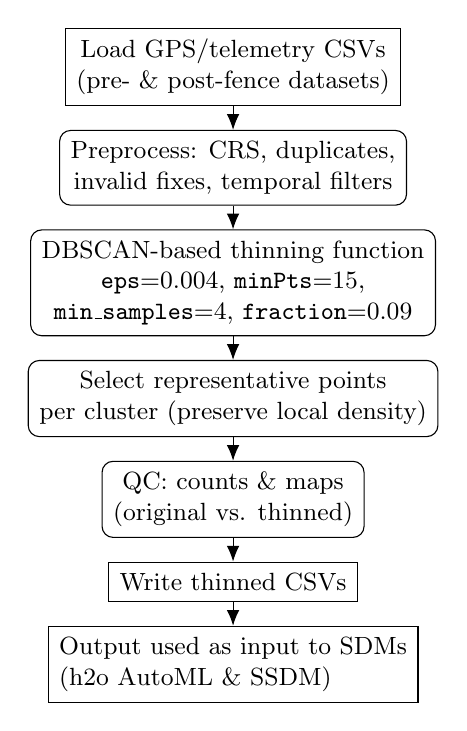
\begin{tikzpicture}[
  node distance=3mm,
  every node/.style={font=\small},
  proc/.style={rectangle, draw, rounded corners, align=center, inner sep=4pt},
  io/.style={rectangle, draw, align=center, inner sep=4pt},
  note/.style={rectangle, draw, align=left, inner sep=4pt},
  >={Latex[length=2mm,width=1.6mm]}
]
% Nodes
\node[io] (load) {Load GPS/telemetry CSVs\\(pre- \& post-fence datasets)};
\node[proc, below=of load] (prep) {Preprocess: CRS, duplicates,\\invalid fixes, temporal filters};
\node[proc, below=of prep] (dbscan) {DBSCAN-based thinning function\\\texttt{eps}=0.004,\ \texttt{minPts}=15,\\\texttt{min\_samples}=4,\ \texttt{fraction}=0.09};
\node[proc, below=of dbscan] (select) {Select representative points\\per cluster (preserve local density)};
\node[proc, below=of select] (qc) {QC: counts \& maps\\(original vs. thinned)};
\node[io,   below=of qc] (save) {Write thinned CSVs};
\node[note, below=of save] (handoff) {Output used as input to SDMs\\(h2o AutoML \& SSDM)};

% Arrows
\draw[->] (load) -- (prep);
\draw[->] (prep) -- (dbscan);
\draw[->] (dbscan) -- (select);
\draw[->] (select) -- (qc);
\draw[->] (qc) -- (save);
\draw[->] (save) -- (handoff);

\end{tikzpicture}%
}
\caption{DBSCAN-based thinning workflow used to reduce spatial autocorrelation and computational load while preserving local density patterns. Parameters were tuned empirically (\texttt{eps}=0.004, \texttt{minPts}=15, \texttt{min\_samples}=4, \texttt{fraction}=0.09).}
\label{fig:dbscan_flowchart}
\end{figure}

\subsection{End-to-end reproducibility}
This project is fully committed to end-to-end reproducibility. All analytical and modelling workflows---from raw data processing and spatial analysis to species distribution modelling, ensemble construction, and visualisation---are thoroughly scripted and versioned. Comprehensive documentation is provided in the project’s \texttt{README.md} and within the code base, all hosted on GitHub (\texttt{https://github.com/[your-repo]}). Each modelling algorithm’s computational time was logged and is reported per model (see Appendix~X). Critically, all final results were generated in \texttt{REPRO} mode, as opposed to \texttt{FAST} mode, to mitigate issues of stochastic randomness and sampling variation between runs. The use of \texttt{renv.lock} ensures strict replicability of the software environment, code, and package versions, so results can be reproduced exactly in the future or by independent researchers. Step-by-step computational workflows, input data, and post-processing scripts are all available, making the entire research process transparent and fully repeatable.

\subsection{Ethical use of AI}
This research adheres to the highest standards of ethical conduct in AI, consistent with Elsevier guidelines and responsible research norms. No images in this manuscript or supplementary materials were generated or manipulated using AI. The first author takes full responsibility for both the accuracy of all research and the ethical standards guiding its presentation. AI tools (\textit{SciSpace}, \textit{Perplexity}, and \textit{Quillbot}) were exclusively used for improving language and readability of the text, while code assistants (\textit{ChatGPT}, \textit{Perplexity AI}) were leveraged to reduce script redundancy and automate R programming tasks, not for data analysis or interpretation. All substantive decisions, analyses, and interpretations remain strictly those of the authors. Furthermore, AI-generated content in this manuscript was independently assessed using the \textit{SciSpace AI Detector}, with an overall detected AI content below 10\% (score: 8\%), underscoring the human-led effort in writing and analysis. No sensitive, proprietary, or personal data was uploaded to or processed by external AI services during any stage of the research.

\end{document}